\chapter{Arquitectura de VirtShell}
\label{Arquitectura}

VirtShell Framework es una plataforma que proporciona herramientas para la automatización y gestión de infraestructura a través del protocolo HTTP \footnote{Hypertext Transfer Protocol o HTTP, es el protocolo de comunicación que permite las transferencias de información en la World Wide Web}. En otros términos, VirtShell facilita la creación, despliegue, mantenimiento y monitoreo tanto de recursos virtuales como físicos por medio de una API REST \footnote{La Transferencia de Estado Representacional (Representational State Transfer) o REST es un estilo de arquitectura software para sistemas hipermedia distribuidos como la World Wide Web.} \cite{fielding00}. Esto permite que cualquier desarrollo de software con acceso a internet (sitio web, aplicación móvil, etc.) pueda utilizar VirtShell e interactuar con la infraestructura tan solo haciendo llamadas a direcciones de internet. \\
\\
VirtShell basa principalmente su funcionamiento en scripts de shell re-utilizables, que facilitan la instalación y configuración de cualquier tipo de servidor o grandes soluciones que involucren varios recursos virtuales sin importar su tamaño. Sin embargo el lenguaje de los scripts no necesariamente debe ser el shell también puede interactuar con cualquier lenguaje de programación que el usuario prefiera.\\
\\
VirtShell es un framework de código abierto y bajo la licencia BSD, que permite utilizarlo para proyectos de cualquier tipo, incluso comerciales. 

\section{Características}

\begin{description}
\item [Programable] VirtShell esta orientado a realizar el aprovisionamiento de sus instancias principalmente por medio de scripts escritos en shell, permitiendo aprovechar todas las estructuras y utilidades del lenguaje de programación. Sin embargo, el lenguaje de shell no es de uso obligatorio, el  metodo de aprovisionamiento puede ser el de la preferencia del usuario. 
\item [Repetible] VirtShell ofrece herramientas para que los scritps de aprovisionamiento sean configurables y  puedan ser ejecutados varias veces en diferentes ambientes de desarrollo o producción.
\item [Modular] VirtShell es un framework organizado de forma modular. Los módulos se encuentran agrupados en categorías que ofrecen las herramientas necesarias para la administración y aprovisionamiento de múltiples recursos virtuales. De igual manera y dada las características de REST, los módulos están diseñados para que se puedan dividir en diferentes servidores obteniendo "micro APIs", lo que permite dividir los procesos y atender diferentes tipos de operaciones del API. 
\item [Escalable] Al ser VirtShell de código abierto, el API puede modificarse, crecer fácilmente y versionarse de diferentes maneras. 
\item [Seguro] VirtShell provee varias capacidades y servicios para aumentar la privacidad y el control de acceso a los diferentes recursos. Los servicios de seguridad permiten crear redes y controlar el acceso a las instancias creadas, así como definir y administrar políticas de acceso a usuarios y permisos sobre cualquier recurso del sistema como por ejemplo scripts de creación y aprovisionamiento.
\item [Extensible] VirtShell fue diseñado con la idea de cargar código dinámicamente, permitiendo extender el comportamiento del framework agregando plugins en tiempo de ejecución.  Adicionalmente VirtShell permite extender el comportamiento del shell desplegando comandos propios que proporcionan ahorro en tiempo y en complejidad.
\item [Inyección de dependencias virtuales] VirtShell adopta la idea del patrón de Inyección de Dependencias \footnote{es un patrón de diseño orientado a objetos, en el que se suministran objetos a una clase en lugar de ser la propia clase quien cree el objeto. El término fue acuñado por primera vez por Martin Fowler.} \cite{fowler04} para conseguir scripts de aprovisionamiento mas desacoplados. De esta manera facilita la configuración de las dependencias que tiene un recurso virtual de otras máquinas virtuales. Para ello, el framework permite declarar el listado de dependencias de recursos virtuales que tiene un script de aprovisionamiento encargándose del correcto acople entre los diferentes recursos virtuales.
\item [Interoperable] Al seguir el estilo arquitectónico REST y contar con la documentación detallada sobre cada uno de los recursos y urls que expone el API de VirtShell, se logra una capacidad clave para la administración remota de la infraestructura virtual. Esta capacidad se refiere al hecho de poder desarrollar aplicaciones en cualquier plataforma y para cualquier dispositivo electrónico, lo que permite funcionar con otros productos o sistemas existentes o futuros.

\end{description}

\section{Módulos}
VirtShell Framework consiste de características organizadas en 13 módulos. Estos módulos son agrupados en Seguridad, Administración y Aprovisionamiento. Estos elementos se usan de manera separada pero trabajan juntos para proveer la información necesaria para que los agentes realicen su trabajo en los hosts que albergaran los recursos virtuales, como se muestra en la figura \ref{fig:framework}. \\

\begin{figure}[h]
    \centering
	\caption{Visión general del framework de VirtShell}
	\label{fig:framework}
	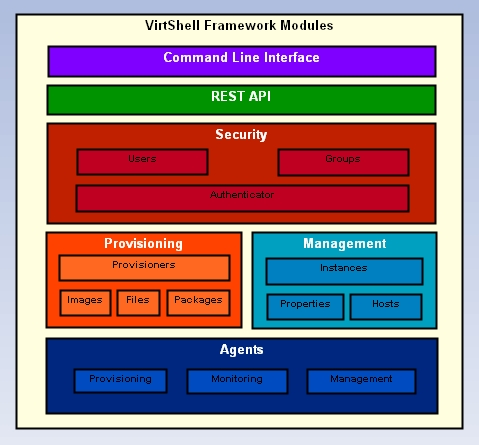
\includegraphics[width = 0.8\textwidth]{../architecture/v1/diagrams/framework}
\end{figure}

Las siguientes secciones detallan los módulos disponibles para cada característica. 

\subsection{Security}
Seguridad consiste de los módulos de usuarios (users), grupos (groups) y el modulo de autenticación (authenticator). El control de los usuarios y grupos son elementos clave en la administración del framework. Los \textbf{Usuarios} pueden ser personas reales, es decir, cuentas ligadas a un usuario físico en particular o cuentas que existen para ser usadas por aplicaciones específicas. \\
\\
Los \textbf{Grupos} son expresiones lógicas de organización, reuniendo usuarios para un propósito común. Los usuarios dentro de un mismo grupo pueden leer, escribir o ejecutar los recursos que pertenecen a ese grupo.\\
\\
El módulo de \textbf{autenticación} soporta el proceso por el cual cuando un usuario se presenta a la aplicación puede validar su identidad. Este módulo es quien decide0 si el usuario tiene permiso para ingresar al sistema y el nivel de acceso a un recurso dado. En el capitulo 4 se detalla el proceso de autenticación y autorización.

\subsection{Managment}
Administración consiste de los modulos anfitriónes (hosts), particiones (partitions), ambientes (enviroments), instancias (instances), propiedades (properties) y tareas (tasks). \\
\\
El módulo de \textbf{anfitriónes} lleva registro de nodos físicos, servidores o máquinas virtuales, que se encuentren conectados a la red y que permitan albergar instancias virtuales. Los anfitriónes son clasificados de acuerdo a diferentes combinaciones de CPU, memoria, almacenamiento y capacidad de trabajo en red, dando flexibilidad para elegir la opcion mas adecuada para las necesidades de las aplicaciones destino. En otras palabras el tipo de anfitrión determina el hardware del nodo físico que sera usado por los recursos virtuales.\\
\\
El módulo de \textbf{particiones} permite dividir los anfitriones en secciones aisladas de disponibilidad. Cada partición puede ser usada para definir áreas geográficas separadas o simplemente para dividir los nodos físicos en subgrupos destinados a diferentes usos o equipos de trabajo o tipos de clientes.\\
\\
El módulo de \textbf{ambientes} permite dividir lógicamente una partición en subredes de trabajo más pequeñas, con lo que se crean grupos más pequeños con diferentes fines. En los ambientes de trabajo se configuran los usuarios que tienen permiso para interactuar trabajar con el.\\
\\
El módulo de \textbf{instancias} es un recurso virtual o máquina virtual o contenedor con parámetros y capacidades definidas en la cual se puede instalar el software deseado. Un usuario puede crear, aprovisionar, actualizar y finalizar instancias en VirtShell tanto como necesite dando la sensación de elasticidad \footnote{La elasticidad es una de las propiedades fundamentales de la nube. La elasticidad consiste en la potencia de escalar los recursos informáticos ampliándolos y reduciéndolos dinámicamente.} de la red.\\
\\
El módulo de \textbf{propiedades} permite consultar información de sistema, de las instancias o de los anfitriones físicos. La información que puede ser consultada es toda aquella que el sistema tenga disponible o que se pueda consultar por medio de comandos de sistema o comandos propios de VirtShell. Ejemplos de información que se puede consultar por medio de las propiedades es porcentajes de memoria y cpu usada, numero de procesos en ejecución, etc. Las propiedades pueden ser consultadas en una sola maquina, o simultáneamente en varias maquinas, o a un conjunto de maquinas de acuerdo a prefijos en su nombre.\\
\\
Finalmente, el módulo de \textbf{tareas} da la información y estado sobre las diferentes tareas o trabajos ejecutados en el sistema. Debido a que el medio para interactuar con los módulos de VirtShell es a través de un API REST, una petición de creación de un nuevo recurso virtual, puede ser largo si el aprovisionamiento involucra varias maquinas. Para evitar, tener una petición esperando respuesta, VirtShell crea una tarea que sera ejecutada de manera asincrónica, dando como respuesta, un identificador de la tarea, para que esta pueda ser consultada posteriormente y conocer el estado de la petición.


\subsection{Provisioning}
Aprovisionamiento consiste de los módulos aprovisonadores (provisioners), imágenes (images), archivos (files) y paquetes (packages).\\
\\
El módulo de \textbf{aprovisionadores} define un marco de aprovisionamiento de un recurso virtual y contiene las configuraciones necesarias para apoyar ese marco. La configuración fundamental de un aprovisionador, es la ruta del repositorio git \footnote{git es un software de control de versiones diseñado por Linus Torvalds}, donde se encuentran los scripts y archivos necesarios para realizar el aprovisionamiento. Del mismo modo la forma de ejecutar los scripts, hace parte de la configuración básica. Para ser mas ligero a VirtShell, los scripts de aprovisionamiento, deben estar registrados en un repositorio git publico. VirtShell se encarga de descargar el repositorio y de ejecutar los scripts de aprovisionamiento, de acuerdo a la configuración especificada. \\
\\
Adicionalmente, los aprovisonadores cuentan con una manera de especificar las dependencias del nuevo recurso virtual. VirtShell se encarga de resolver las dependencias antes de realizar el aprovisionamiento del nuevo recurso, a su vez, suministra información de ellas a los scripts de aprovisionamiento si estos lo requieren. \\
\\
VirtShell utiliza como lenguaje de referencia, para la creación de scripts de aprovisionamiento, el lenguaje shell. Este cuenta con los recursos suficientes para interactuar con los diferentes sistemas operativos de las instancias. Sin embargo estos comandos se pueden extender usando el paquete de comandos propios de VirtShell, los cuales pueden abstraer muchas de las operaciones del shell. Esto facilita la escritura de los mismos o permite hacerlos independientes del sistema operativo en el cual van a ejecutarse.\\
\\
El módulo de \textbf{imágenes} proporciona la información necesaria de las imágenes que se encuentran registradas en el sistema. Cada vez que se crea un nuevo recurso virtual en un anfitrión, se especifica el nombre de la imagen almacenada en el sistema que sera usada, de una de las que se encuentra en el sistema. \\
\\
Las imágenes que se manejan en VirtShell son de dos tipos: ISO \footnote{Una imagen ISO es un archivo informático donde se almacena una copia o imagen exacta de un sistema de archivos o ficheros de un disco óptico, normalmente un disco compacto (CD) o un disco versátil digital (DVD).} y para contenedores. Las de tipo ISO, se encuentran guardadas en el repositorio de VirtShell, y su uso se enfoca a maquinas virtuales que interactuan con hypervisors. Las imágenes de tipo contenedor, se emplean para tecnologías de visualización de sistema operativo como LXC y Docker. Estas son descargadas automáticamente de los repositorios de dominio publico de los diferentes proveedores. \\
\\
El módulo de imágenes cuenta también, con la característica de crear automáticamente nuevas imágenes de tipo ISO a partir de las \emph{releases} (liberaciones) base de las diferentes distribuciones de sistemas operativos linux. Una vez creada la nueva ISO esta sera guardada en el repositorio interno para su posterior uso.\\
\\
El módulo de \textbf{archivos} proporciona una manera de enviar archivos a uno o mas recursos virtuales de manera simultanea en un directorio especificado. Adicionalmente, permite especificar los permisos que tendrán los archivos. Cabe anotar, que  estos deben estar previamente almacenados en el sistema.\\
\\
El módulo de \textbf{paquetes} facilita realizar funciones tales como la instalación de nuevos paquetes de software y actualización de paquetes existentes en uno o mas recursos virtuales de manera simultanea.


\subsection{Agents}
Los Agentes son servicios que se ejecutan localmente en cada anfitrión, y que se encuentra bajo la gestión de VirtShell. Estos actúan con un cierto grado de autonomía con el fin de completar tareas en nombre del servidor.\\
\\ 
VirtShell, cuenta con tres tipos de agentes: de aprovisionamiento, monitoreo y administración. El agente de aprovisionamiento es de tipo reactivo y se encarga de dar respuesta a todas las peticiones de aprovisionamiento sobre uno o mas recursos virtuales en el anfitrión.\\
\\
El agente de monitoreo es completamente autónomo. Su función es la de supervisar al agente de aprovisionamiento, y reportar el estado de salud de los anfitriones y recursos virtuales que se encuentran creados en su interior.\\
\\
El agente de administración se encarga de gestionar las instancias, permite detener, iniciar, clonar, eliminar y obtener información especifica de cada instancia que se ejecuta en el anfitrión.\\
\\
Los agentes son instalados de manera automática en el anfitrión cuando este es agregado al sistema por medio del API REST, liberando de esta tarea al administrador del sistema.

